% !TEX root = ../thesis.tex

\chapter{Syncer Optimisations}
In this chapter, we improve on the initial design of the framework described in chapter \ref{cha:design_implementation}. We run benchmarks on the optimisations proposed, and present the results. The specifications of the two setups used for testing are shown in table \ref{table:benchmark-specs}.

\begin{table}[H]
  \centering
  \begin{minipage}{0.45\textwidth}
  \begin{tabular}{|r|l|} \hline
    \multicolumn{2}{|c|}{\textbf{MacBook Pro 2011 (MBP)}} \\ \hline
    \textbf{OS} & OS X 10.10.4 (Yosemite)\\ \hline
    \textbf{Processor} & 2.3 GHz Intel Core i5\\ \hline
    \textbf{Memory} & 8 GB 1333 MHz DDR3 \\ \hline
    \textbf{Storage} & 256GB SSD Crucial m4\\ \hline
    \textbf{Network} & 24.4/2.5 kbps VDSL line\\ \hline
  \end{tabular}

  \end{minipage}
  \begin{minipage}{0.45\textwidth}
  \begin{tabular}{|r|l|} \hline
    \multicolumn{2}{|c|}{\textbf{\textasciitilde okeanos Virtual Machine (VM)}} \\ \hline
    \textbf{OS} & Ubuntu Linux 14.04.2 LTS (Trusty)\\ \hline
    \textbf{Processor} & 2.1 GHz Virtual CPU QEMU v2.1.2 \\ \hline
    \textbf{Memory} & 4 GB Virtual RAM \\ \hline
    \textbf{Storage} & 80 GB (DRBD) \\ \hline
    \textbf{Network} & TODO: Network \\ \hline
  \end{tabular}
  \end{minipage}
  \caption{Benchmark setups specs}
  \label{table:benchmark-specs}
\end{table}

\end{tabular}

\section{Request queuing}
  After using the framework with the help of a profiler, it became apparent that a bottleneck existed whenever there was a need for multiple requests on the remote server, due to the latency and the round-trip times. Additionally, during the transfer (download or upload) of a large file, the synchronisation process was being unnecessarily stalled until the tranfer finished. To overcome these issues, a request queuing system was implemented, dispatching the requests to different threads, while the main thread continued the execution of the sync. There was also a dramatic speedup when step 2 of the syncing algorithm was modified to request all objects' metadata from the remote server together, instead of individually for each file. To ensure correctness in the synchronisation process, the program should wait until all threads executing requests for a step of an algorithm (as described in section \ref{ssec:3step_algorithm}) have finished, before starting a different step. A more efficient solution would be to implement a locking mechanism and disallow actions on files already being processed by a spawned thread, but this would require substantial changes in the framework code.
  \subsection{Benchmarks}
    \subsubsection{Upload time relative to number of threads}
      For the first benchmark, we tried to upload 100 files of 150 bytes each sequentially (denoted as ``0'' threads in the tables) and again by using a different number of threads. The files were always being randomly generated, because Pithos+ stores the blocks that are uploaded, and we needed to evade that caching for accurate measurements. Each batch of uploads was executed 10 times, and the results presented are the average of those tries. The results are statistically accurate, having a standard deviation of $\sigma_A = 1.1$.
      \begin{table}[H]
        \setlength{\tabcolsep}{12pt}
        \begin{adjustbox}{max width=1.2\textwidth, center}
        \begin{tabular}{c|*{12}{c|}}
          \cline{2-12}
          & \multicolumn{11}{ |c| }{\textbf{\# of threads}} \\ \cline{2-12}
          & \textbf{0} & \textbf{1} & \textbf{2} & \textbf{4} & \textbf{8} & \textbf{12} & \textbf{16} & \textbf{20} & \textbf{24} & \textbf{28} & \textbf{32} \\ \cline{1-12}
          \multicolumn{1}{ |c| }{\textbf{time (s)}} & 72.3 & 72.8 & 43.9 & 34.8 & 32.8 & 33.5 & 34.8 & 33.2 & 33.0 & 34.0 & 32.3 \\ \cline{1-12}
          \multicolumn{1}{ |c| }{\textbf{speedup (\%)}} & N/A & -0.7 & 39.2 & 51.9 & 54.7 & 53.6 & 51.8 & 54.1 & 54.3 & 53.0 & 55.4 \\ \cline{1-12}
        \end{tabular}
        \end{adjustbox}
        \caption{MBP upload speedup by queuing, relative to \# of threads}
        \label{table:mbp-upload-threads}
      \end{table}

      \begin{table}[H]
        \setlength{\tabcolsep}{12pt}
        \begin{adjustbox}{max width=1.2\textwidth, center}
        \begin{tabular}{c|*{12}{c|}}
          \cline{2-12}
          & \multicolumn{11}{ |c| }{\textbf{\# of threads}} \\ \cline{2-12}
          & \textbf{0} & \textbf{1} & \textbf{2} & \textbf{4} & \textbf{8} & \textbf{12} & \textbf{16} & \textbf{20} & \textbf{24} & \textbf{28} & \textbf{32} \\ \cline{1-12}
          \multicolumn{1}{ |c| }{\textbf{time (s)}} & 00.0 & 00.0 & 00.0 & 00.0 & 00.0 & 00.0 & 00.0 & 00.0 & 00.0 & 00.0 & 00.0 \\ \cline{1-12}
          \multicolumn{1}{ |c| }{\textbf{speedup (\%)}} & 00.0 & 00.0 & 00.0 & 00.0 & 00.0 & 00.0 & 00.0 & 00.0 & 00.0 & 00.0 & 00.0 \\ \cline{1-12}
        \end{tabular}
        \end{adjustbox}
        \caption{VM upload speedup by queuing, relative to \# of threads}
        \label{table:benchmark-specs}
      \end{table}

      It is visible that there is a considerable speedup when using multiple threads to upload the files, with the uploads completing in less than half the time on the VM, when 4 or more threads were used.

      %TODO: Benchmarks for large files, many threads fail.

\section{Directory monitoring}
  Detecting file changes on the original algorithm meant that each file in the directory would have to be individually checked for updates, a process that scales linearly with the number of files present. Even at a speed of about 1000 files scanned per second on an SSD (MBP), each sync would need over 100 seconds for the local directory only, which is highly undesirable. The solution to this problem is to use the filesystem monitoring mechanisms that exist for the Operating Systems (OS), to quickly produce a substantially smaller set of files that have potentially changed. Such utilities and functions exist for the most common OS and are:
  \begin{itemize}
    \item inotify (Linux 2.6 or later)
    \item FSEvents (Mac OS X)
    \item kqueue (FreeBSD, BSD, OS X)
    \item ReadDirectoryChangesW function (Windows)
  \end{itemize}

  To implement this in the framework, the \emph{watchdog} Python library was used, which provides easy access to the aforementioned utilities. Two functions, \emph{start()} and \emph{stop()} were added to the LocalDirectory class, and then inherited to the WatchdogDirectory subclass. Those two functions are a no-op in the original implementation. To avoid the risk of an incorrect synchronisation if some files were modified while the monitoring was not active, the framework always perform a full local scan on startup, using the \emph{get\_all\_objects\_fstat()} function, and uses the more efficient \emph{get\_modified\_objects\_fstat()} for all subsequent scans, while the application remains active.

  \begin{figure}[H]
    \centering
    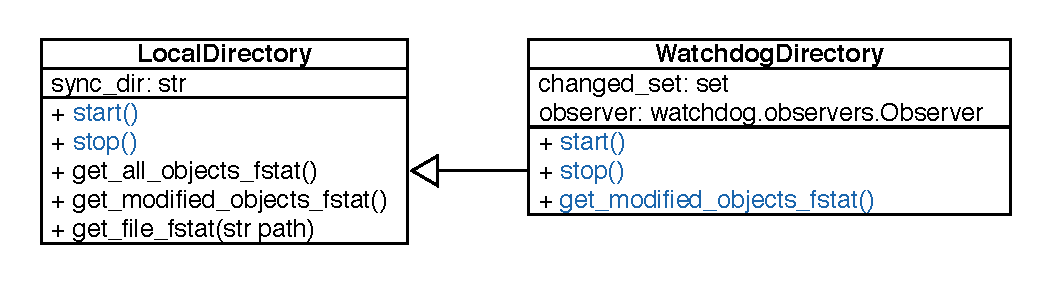
\includegraphics{Images/WatchDir.eps}
    \caption{WatchdogDirectory}
    \label{fig:watchdir_uml}
  \end{figure}

  \begin{itemize}
    \item \textbf{changed\_set}: The set containing all files that were created, modified or renamed, since the last time \emph{get\_modified\_objects\_fstat()} was called.
    \item \textbf{observer}: The thread that monitors the sync directory for changes.\\

    \item \textbf{start}: Starts the observer thread.
    \item \textbf{stop}: Stops the observer thread.
    \item \textbf{get\_modified\_objects\_fstat}: Returns the metadata of the files in the \emph{changed\_set} as FileStat objects. Clears the \emph{changed\_set}.
  \end{itemize}

  \subsection{Benchmarks}
  bench

\section{Local block storage}
  TODO: Local block storage + benchmarks
  \subsection{Benchmarks}
  bench
